\section{Implementation}\label{sec:impl}

%* Discuss how formulas are interpreted / parsed into tree-structures where each the nodes themselves 'contain' definitions for the semantics behind the logical connective they represent, based on their class.
%* Refer back to previously presented algorithms when discussing recursive checking function
%* Refer back to background chapter when discussing why the problem is interesting when presenting artifact.
%* Model checking often limited to yes / no questions, discuss added value by transcending boolean 

%JFLAP, a tool previously used here at our faculty to teach students how turing machines and finite state automatas work.

%Innholdsliste:

%Recap motivasjon
%Forklar hvorfor grensesnittet ble som det ble, inspirasjon fra JFLAP ect
%Anekdote rundt bruken av JFLAP 
	%Nytte for studenter
%Introduksjon til visualisering, vis basics
	%Trekke sammenligninger mellom visualiseringen av Kripke og FSAer
%Diskuter tegning av modeller, tilstander, kanter og agenter
	%Grunngi 
%Nevn håndtering av props og agentlister

%Vis eksempler på sjekking av basic formler
%Forklar innlesing av formler
%Diskuter forskjeller mellom innskreven form vs logiske symboler (enklere å skrive inn)
%Forklar hva som skjer, først sjekk hvilke states i modellen
%Nevn interaktivitet gjennom sjekke subformler ved å muse over

%Diskuter motivasjon og hensikt bak stepping-funksjonalitet
	%	Sammenlign med stepper i JFLAP
%Vis basic eksempel på hvordan verktøyet presenterer steg-loggen
%Vis mer avansert eksempel med public announcements og modell-oppdateringer
%Vis eksempel med group announcements og hvordan verktøyet visualiserer de ulike strukturene koalisjoner kan begrense den orginale modellen til
	%	Muligens visualisere kunnskap de dicto vs de re? Må finne enkelt eksempel som ikke blir horribelt rotete i så fall


In this chapter we will present our own implementation of a model checker for Group Announcement Logic called \cname{} and describe its inner workings. Our initial goal with \cname{} was to create an educational tool that could aid students with learning epistemic logic in a more visual manner. Therefore, while most other model checking utilities such as DEMO \cite{JanvanEijck} stick to answering the user's queries with simple yes and no answers, we wanted to go beyond that by showing them not just whether their formulas hold, but also visualize why and provide the user with an easier, visual way of drawing models almost as they would on paper or blackboard. The reasoning behind this was that by allowing the user to manipulate the model through a simple click-and-drag interface and seeing how it can affect the valuation of various formulas they might gain a deeper understanding of the semantics involved.

One of the big questions that needed to be answered when we started building \cname{} was how we wanted to not just present and visualize these highly abstract models, but also allow the user to manipulate them in a way that would be intuitive and easy to grasp. As I had previously used a tool called JFLAP\footnote{www.jflap.org} with great success when teaching students as a TA about Turing machines and finite state automata (FSAs) I ended up drawing most of my inspiration from it when drawing up my initial sketches for how I imagined my own tool might look. While my own experience with JFLAP is mostly limited to visualizing, editing and toying with Turing machines and finite state automatas, it is a fairly sophisticated package of graphical tools covering also covering many other concepts of formal languages and automata theory. JFLAPs editor is relatively simplistic, but it still helped my own and my students' understanding of FSAs tremendously by allowing us to interact and play with what is otherwise a really abstract concept and as such, I wanted to see if I could create a similarly potent learning aid for epistemic logic. 

\begin{figure}[H]
	\label{fig:JFLAP_basic illustration}
	\caption{A basic two-state turing machine}
	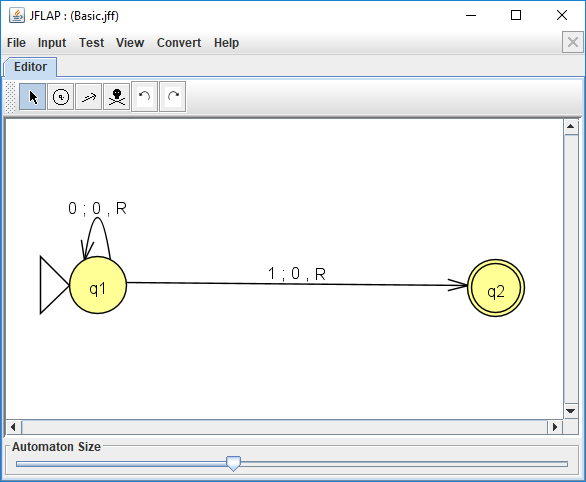
\includegraphics[width= \textwidth]{JFLAPbasicIllustration.PNG}
\end{figure}

%When I took the same course myself the year before I became a TA in it, most of the students, myself included found Turing machines to be a really hard and abstract concept to grasp as we were simply explained how they worked and then instructed to write instructions that would perform certain basic tasks using pen and paper alone. Obviously, this left us without any way to check whether or not our 

While I could have created a simpler non-graphical model checking tool for GAL similar to DEMO, I wanted to create something more powerful that could help visualize epistemic logic the same way that JFLAP visualizes Turing machines. This ended up taking a lot of work, but my justification is that although a similar non-graphical tool would probably have helped me teach my students how FSAs and Turing machines work as well, I highly doubt it would have been anywhere near as effective without being able to visualize the 'how's and 'why's and instead only spat out 'yes' or 'no' answers to our queries in the same manner that most model checking utilities do. 
%Learning benefit

\subsection{Visualization of Kripke structures}
%Visualization of Turing machines vs kripke stuctures
%Both have states, transitions vs indistinguishability, tape of input vs formula to traverse and check
Although finite state automatons and epistemic logic might initially seem relatively far detached, the Kripke structures we use share a fair few similarities to FSAs that made me realize I could visualize our models in almost the same manner as JFLAP does its automatons. For instance, they both consist of a set of states, and while FSAs and Turing machines have transition rules, whereas we have an indistinguishability relation, they can both basically just be visualized as edges in a graph where the nodes are our states. Whereas JFLAP labels its edges with the each transition rule, we label ours with the set of agents that considers our pair of states indistinguishable and additionally label each state with the set of propositions that hold in it. We present our tool visualizing a basic model in Figure \ref{fig:basicModelVis}.


\begin{figure}[H]
	\label{fig:basicModelVis}
	\caption{A basic model, visualized in \cname}
	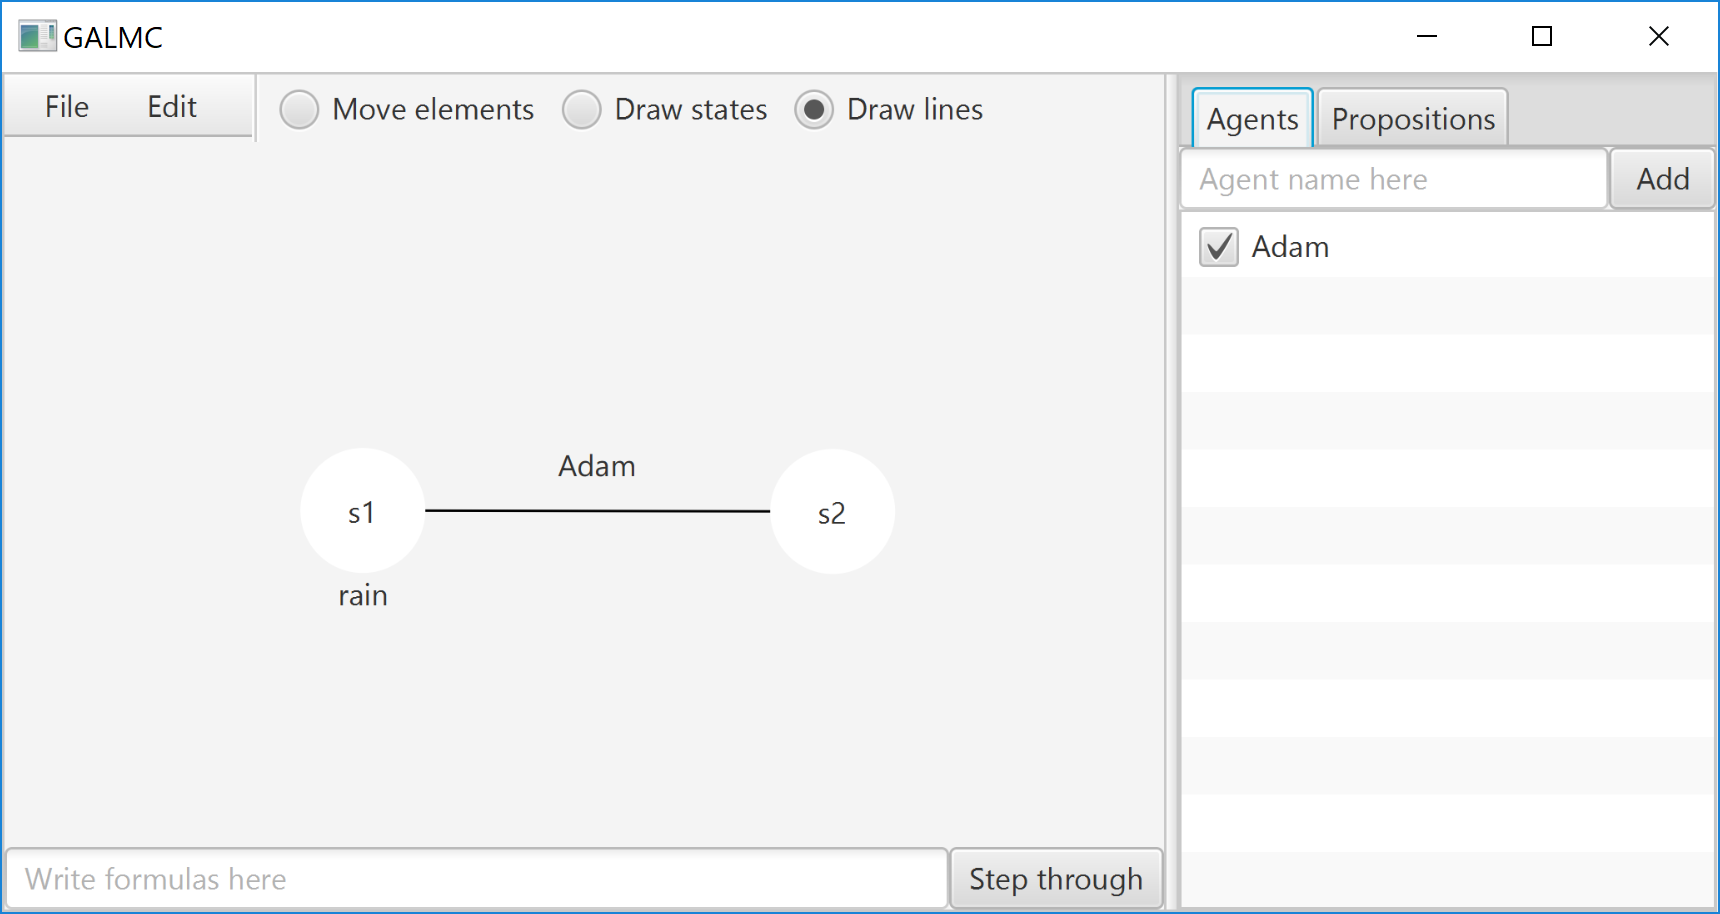
\includegraphics[width= \textwidth]{BasicModel.png}
\end{figure} 

%Mention basic usage, how one draws models, example blackboard, simple, intuitive, easy
As can be seen in Figure \ref{fig:basicModelVis}, the UI of \cname{} is fairly close to that of JFLAP, as I wanted to recreate its way of drawing models almost as one does with pen and paper as much as possible so that the interface feels `natural' and intuitive to someone with little to no previous experience with Kripke structures. As such, the editor was made to be as simple as possible, consisting of only three main tools, one for selecting and moving elements, one for drawing new states and one for creating edges between them. Additionally, the editor provides two side panels for managing the lists of properties and agents in our models, where the we can also select which ones to use when drawing new components or to apply to existing ones.

After the user creates their model, the next step is to start checking formulas against it. One trade-off that had to be made here was whether or not to stick to the original symbols for the various operators in our language or to come up with replacements which are easier to type in. As requiring the user to memorize half a dozen unicode character codes probably would not offer the best user experience, I opted to replace them with more easily accessible replacements I figured would make sense to most users. Since I assume most users of my users to be at least faintly familiar with programming, I ended up taking most of my inspiration from symbols used to represent boolean operators in programming, such as replacing $\vee$ and $\cup$ with $\|$ and $\&$ for disjunctions and conjunctions respectively, as they can basically be seen as `or' and `and'. That said, the editor helpfully translates any formula the user types in back into proper legal formulas when displaying them, which should hopefully clear up any confusion, at least once the user looks up which symbols were replaced \footnote{For the full list of replaced symbols and their replacements, see the tool's wiki pages at https://github.com/AndersKaareEide/MCGAL/wiki}.

%Checking formulas, visualize which states in our model satisfy the given formula
%Mention interactive formula display with subformulas

When the user finishes typing in their formula, the tool checks their formula against each state in their model and colors each state based on whether or not the user's formula is satisfied in that state, which can be seen in Figure \ref{fig:labelHover}.

\todo{replace image with one that shows mouse pointer}
\begin{figure}[H]
	\label{fig:labelHover}
	\caption{Illustration of interactive formula display}
	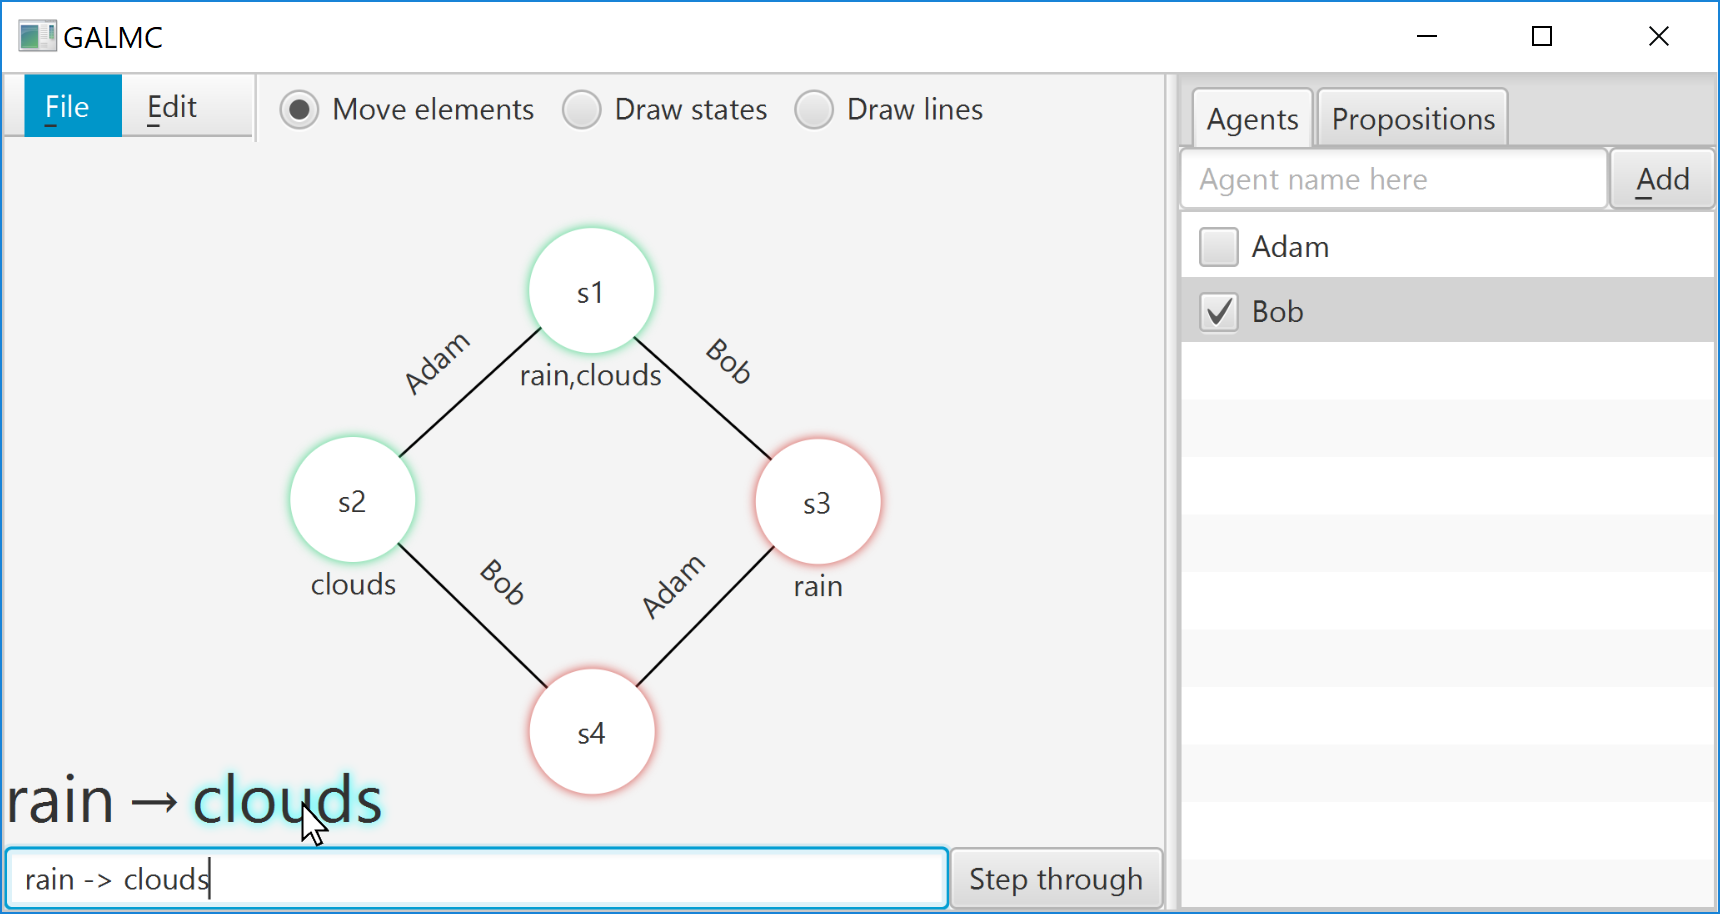
\includegraphics[width= \textwidth]{LabelMouseOver.png}
\end{figure}
%Paint models, states

%Mention deviation from logic here? Flipped valuation function, 

\subsection{Generating examples}
%Move to wayyyy later
As our motivation behind creating \cname was to create a learning tool that could help new logicians understand how the semantics of GAL work, being able to generate examples which highlight interesting properties of our models is highly important. As such, MCGAL was designed from the ground up to be able to trace its steps through the model checking process so that it can also display each step of this process in an intuitive manner. The program therefore creates a log entry each time it checks an operator against a specific state in the model, keeping track of sub-formulas and formula depth as it goes through the operators. The reason behind also keeping track of sub-formulas and formula depth in the logs is to create a more easily navigable tree-like structure. This tree-structure facilitates skipping through chunks of the process that might not be particularly interesting to the user, allowing them to for example view each state the tool checks against a particular K-operator, or even skip through each of the possible updated models a coalition can reduce a model to through their announceable extensions, without having to step through the checking of the inner formula every time.
 
\begin{figure}[H]
	\label{fig:basicGalChecking}
	\caption{Checking a basic group announcement formula in MCGAL}
	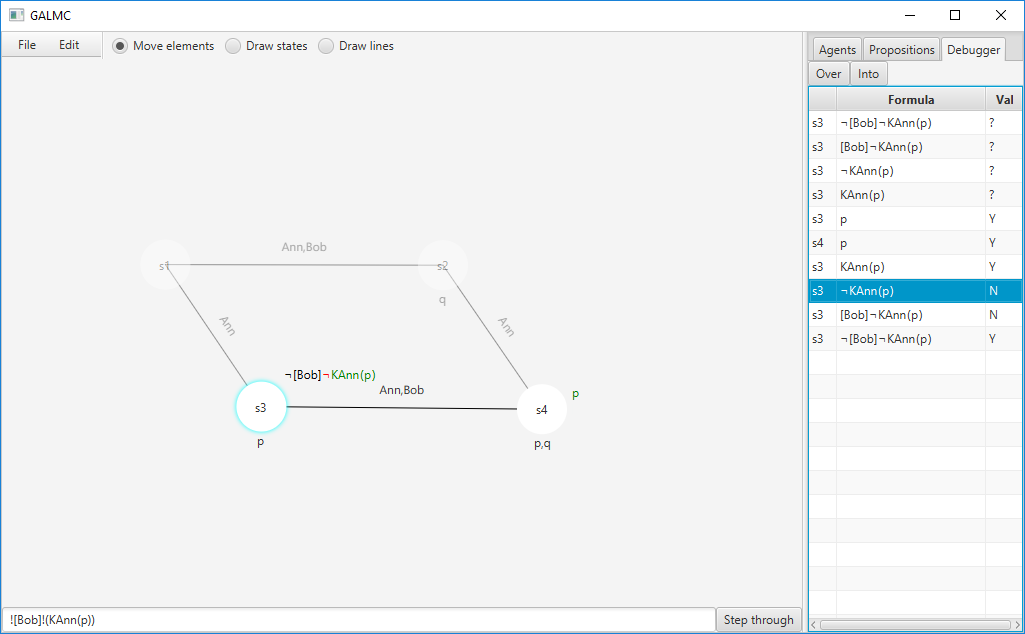
\includegraphics[width= \textwidth]{MCGALBasicChecking.png}
\end{figure}

As the tool provides a view of the model, it also updates this view by showing what the model it is currently checking against looks like, by highlighting the state and operator the tool is currently checking as well as graying out any states that have been filtered out by model updates. Examples of such model updates might be constraining the model to one of the formula extensions a coalition can announce, which is what is being displayed in Figure \ref{fig:basicGalChecking}. In this example, we are checking whether the formula $\neg [Bob]\neg K_{Ann}[p]$ holds in state s3 of our model. The formula roughly translates to: 'It is not the case that Bob is unable to make Ann know $p$' or more simply in its dual form: 'Bob is able to make Ann know p'. From the visualization of our model in Figure \ref{fig:basicGalChecking} we can see that since Bob is able to reduce the model to only states where $p$ holds, Ann also trivially knows that $p$ holds in this updated model, satisfying our original formula. In this somewhat trivial example, the tool ended up only having to try announcing a single formula extension before it found an extension that made our original formula true. If we were to check a more complex formula however, it might end up checking tens of different announcements, each generating a different updated model after its announcement which the tool will helpfully visualize, giving the user insight into a coalition's capabilities. Note that the previous example could also have been made easier by rewriting the formula as $\dia{Bob}K_{Ann}[p]$, but unfortunately the tool does not (yet) support diamond operators. 


\begin{figure}[h]
	\label{fig:debugExmpl}
	\caption{Example of using \cname's step-by-step formula checking}
	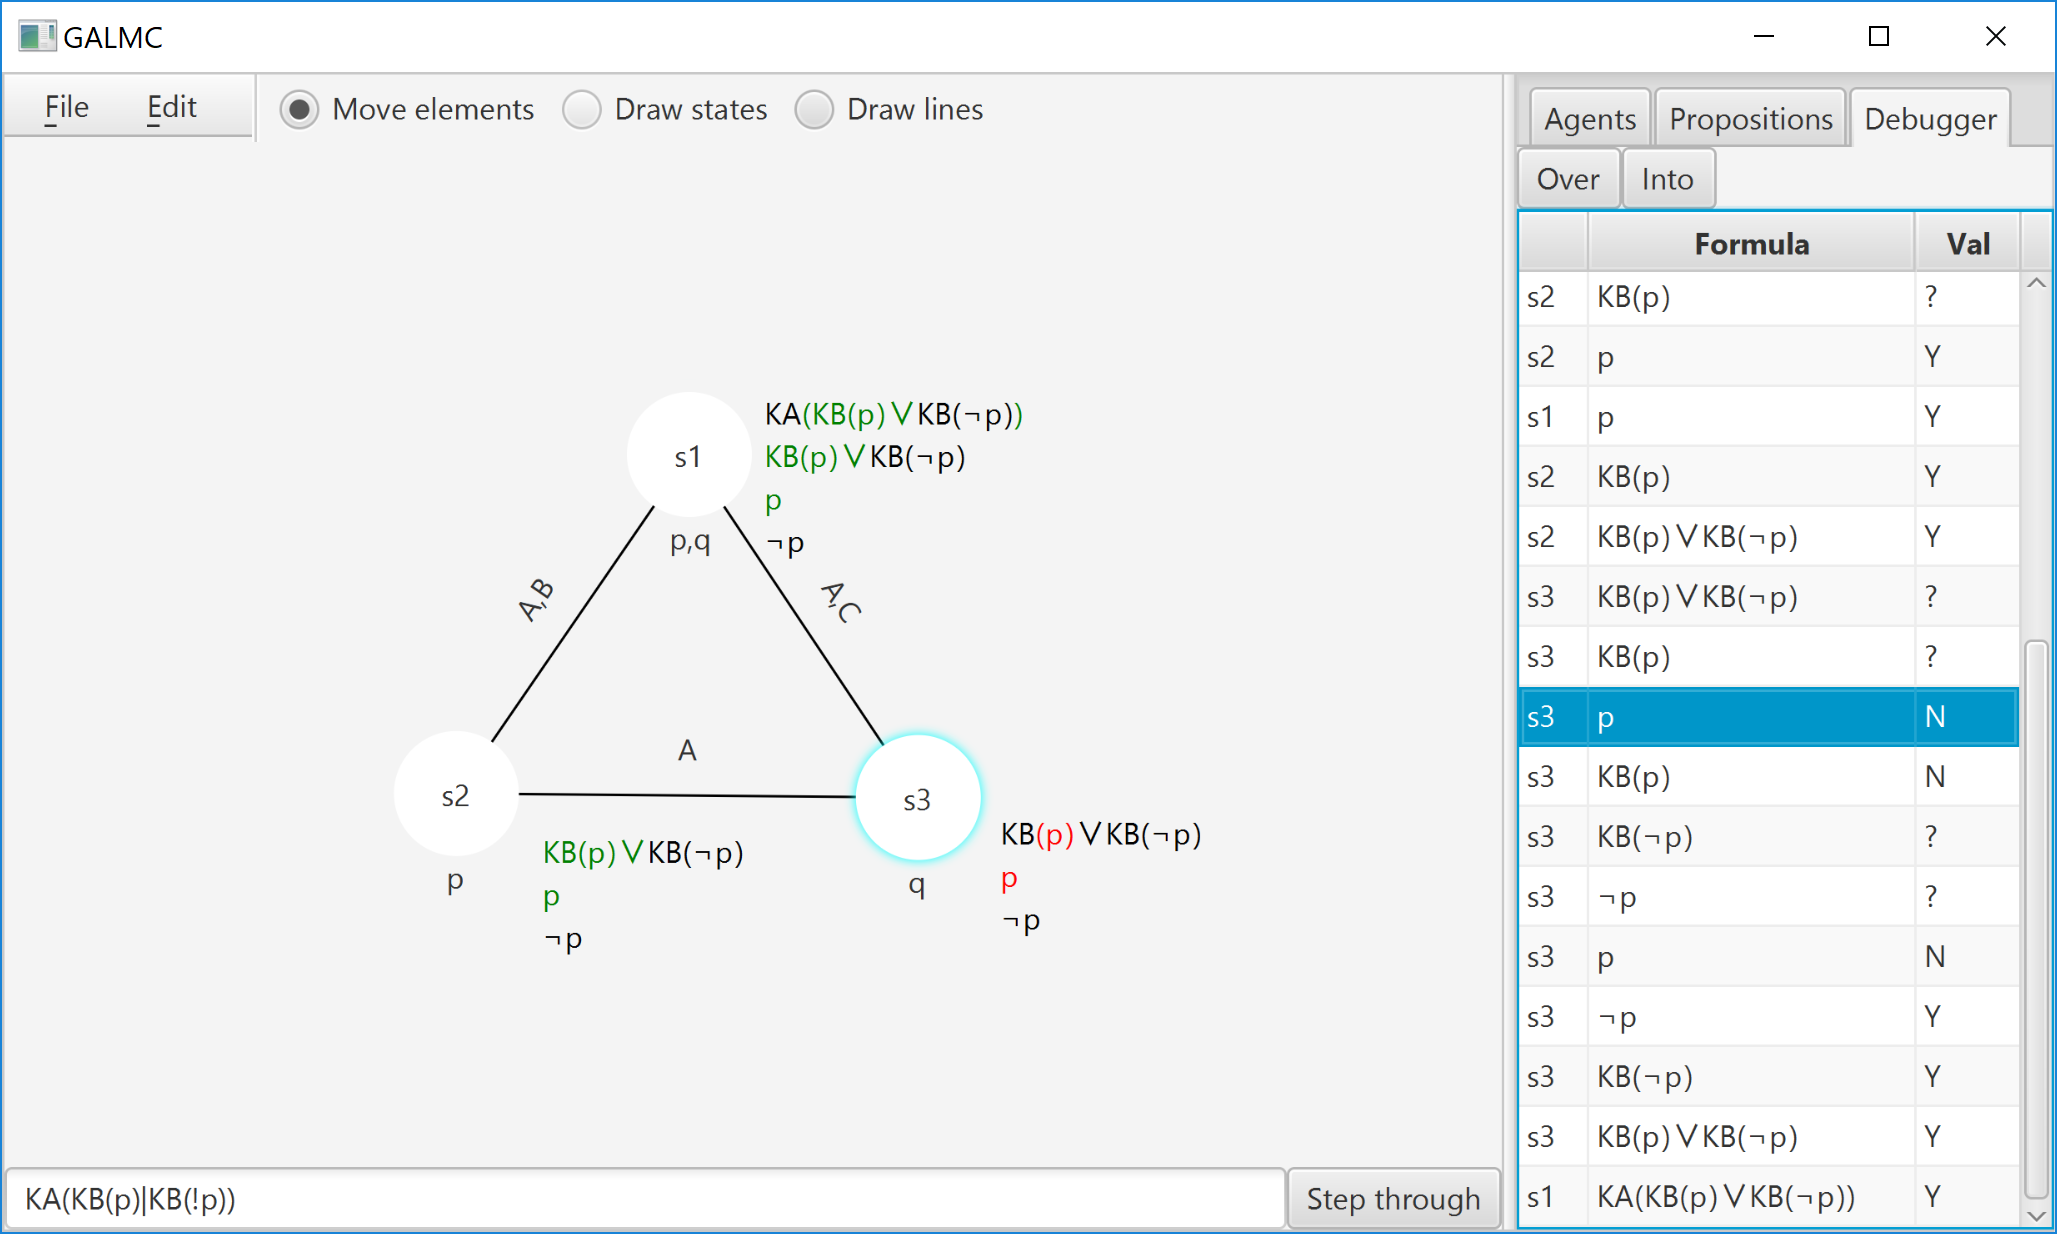
\includegraphics[width=\textwidth]{DebuggerExample.png}
\end{figure}

%Admittedly UX and design in general is not my strong suit and improving the interface is left as future work
%They would additionally be able to type in a formula and then have the states in their model light up, highlighting which states satisfy the given formula. 

Another key feature of the application is that it also helps the user keep track of which formulas are being checked in the various states, by displaying the formulas as a list next to each state and coloring them by their valuation as the user steps through the checking process.  addition to simply checking which states in the user's model satisfy their fomula, they can also look more closely at why a formula is or is not satisfied in a given state. In order to help the user with this, the application visualizes the checking process step-by-step, one operator and state at a time, with progress being displayed by updating the color of each operator in the formula according to their current valuation.


Figure \ref{fig:debugExmpl} shows a screenshot of \cname in action, where the user is stepping through the process of checking a specific formula against a state in their model, having the tool visualize whether or not their formula holds. It also shows how the application breaks down epistemic formulas into sub-formulas and display them next to each state they have to be checked in. Additionally, the application also visualizes the current valuation of each operator and proposition in the formula as you step through the checking process, as can be seen from the red and green parts of the formulas being checked, as well as the Val column in the debugger tab. Note that the user can also step forwards or backwards through this process at any time by either clicking the step they want to skip to, or browsing with the arrow keys. 


\subsection{Choice of platform}

\subsection{Language and interpretation}

\subsection{Model checking}


\subsection{Tech choices}

Our model checker was implemented in Kotlin as it is a new and exiting language while also being based on the JVM, providing access to the wast libraries and tools written for Java, including JavaFX and a Java hook for ANTLR which will be discussed in more detail later in this section. Kotlin additionally has a smooth and concise syntax as well as lending itself very well towards writing functional code despite being object oriented through shorthands for lambda expressions, support for proper function types and distinctions between mutable and immutable structures and variables. Among the other benefits of the language is that Kotlin being a relatively fresh and recent language, is that it has been able to draw plenty of inspiration from other  meaning it also has lots of lovely `modern' language features such as type inference, string interpolation and default values for making function arguments optional, meaning you no longer have to write three different constructors as one would in good old Java. While the language is still relatively young, being first unveiled in 2011\cite{KotlinHello}, it is being backed by Jetbrains, who are well known for their suite of plugins and IDEs such as IntelliJ and PyCharm, meaning the language has excellent tooling support despite its young age.

As for the choice of graphics library to build the application's user interface in, the choice fell on a Kotlin wrapper for the de facto standard Java GUI library of JavaFX, called TornadoFX\footnote{Library homepage at: \url{https://tornadofx.io}}. While JavaFX is a widely used and mature library with powerful features, we also feel it tends to be somewhat clunky and verbose unless one dumps the layout and positioning of components into specialized XML-files. While this helps clean up classes representing UI-components, we also find it makes dynamic component generation clumsier. Our reasons for wanting to use TornadoFX over plain JavaFX is that TornadoFX, being a Kotlin library is able to have a much cleaner and prettier API by utilizing Kotlin features such as lambda expressions attached to receivers to create composable builder functions which generate your JavaFX component hierarchy in an imperative fashion. Another excellent feature of TornadoFX is its concise shorthands for creating dynamic bindings between UI components and observable sets of data. An example of this would be using the standard bindChildren() function to dynamically create and destroy UI components representing states in the user's epistemic model based on changes to that internal list of objects which represent states in a single line of code, by simply feeding the bindChildren() function a reference to the observable list of states and a transformation function that converts the data structure representing a state, to the corresponding UI component, in our case simply the constructor of this component. If anything, I would say that TornadoFX's greatest feature is how its composable builder functions allows you to circumvent the normally inverse order of declaration and creation of UI components compared to their order in the component hierarchy, which can be seen in Figure \ref{fig:StatFragSnip}. \todo{Find out why Latex is fucking up this reference}

\begin{figure}[h]
	\label{fig:StatFragSnip}
	\caption{Code handling how the UI components representing states are built. Note the conciseness due to implicit contexts.}
	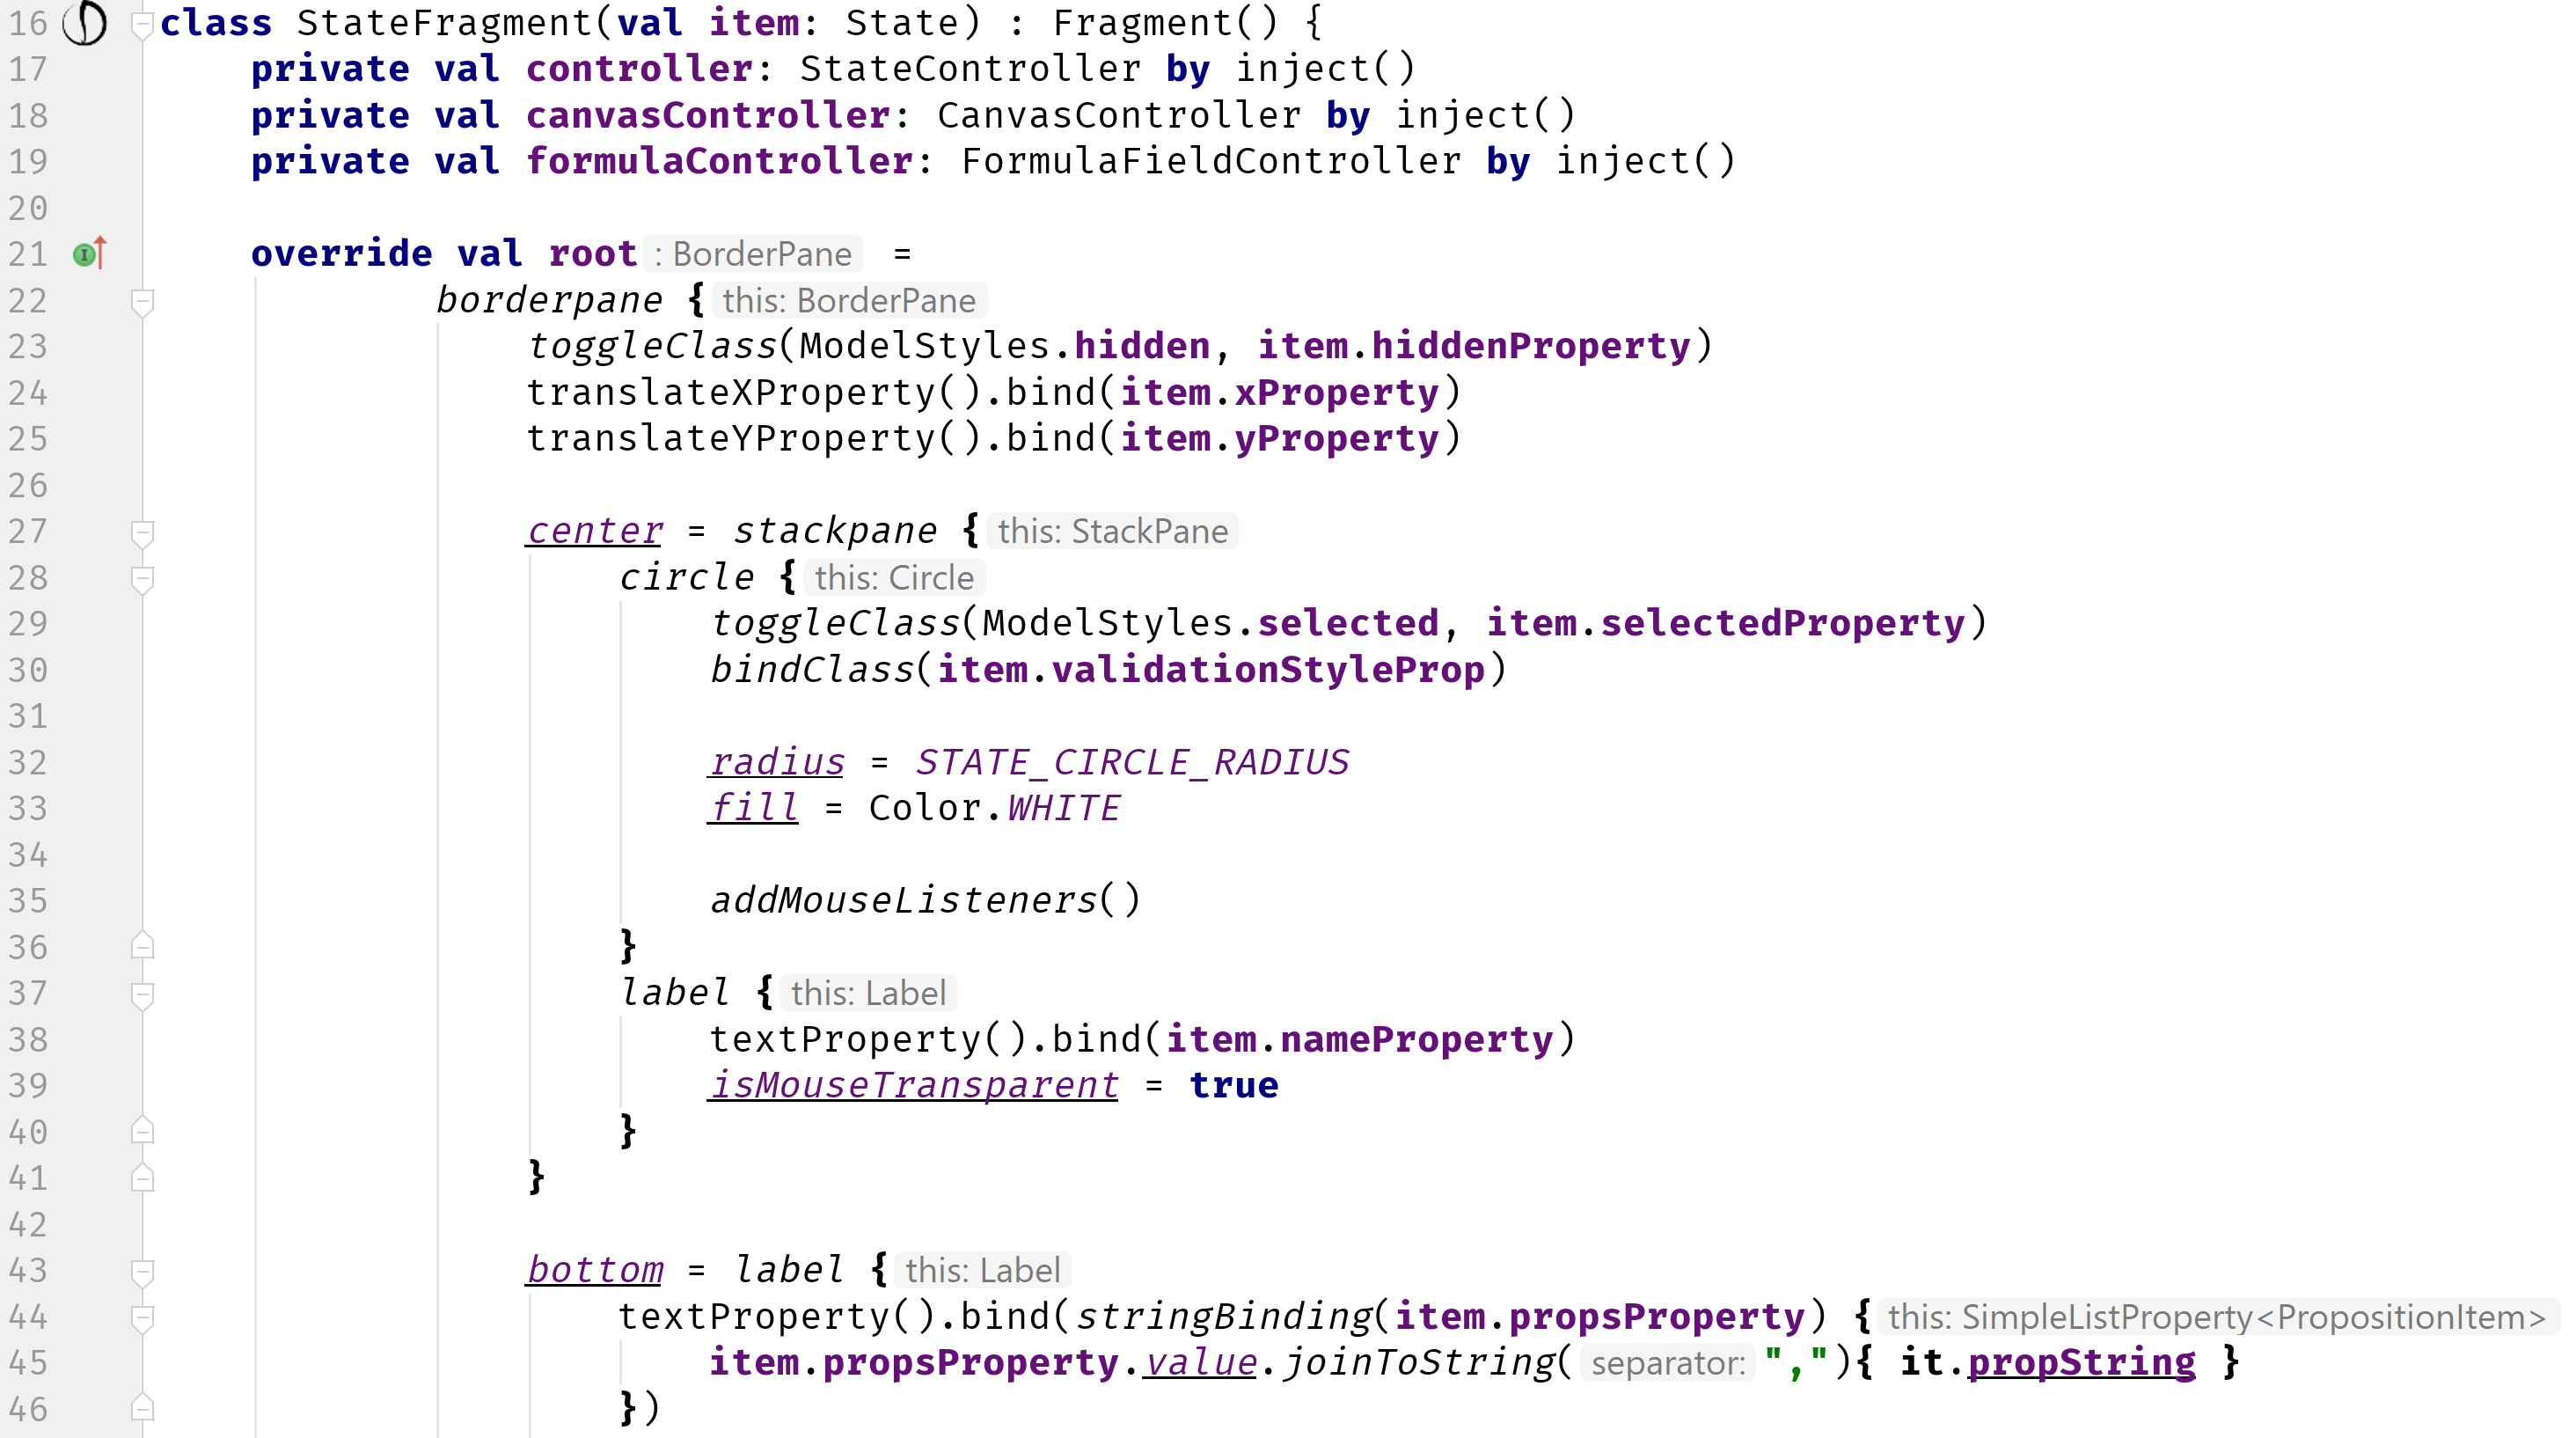
\includegraphics[width=\textwidth]{StateFragmentSnippet.png}
\end{figure}

As for parsing the formulas, I went with ANTLR\footnote{\url{http://www.antlr.org/}} for generating the parsers I needed. ANTLR is a pretty powerful tool for generating parsers and lexers based on easily definable grammatical rules like the ones in Figure \ref{fig:grammar}

\begin{figure}[h]
	\label{fig:grammar}
	\caption{Grammatical rules for parsing formulas in \cname with ANTLR. }
	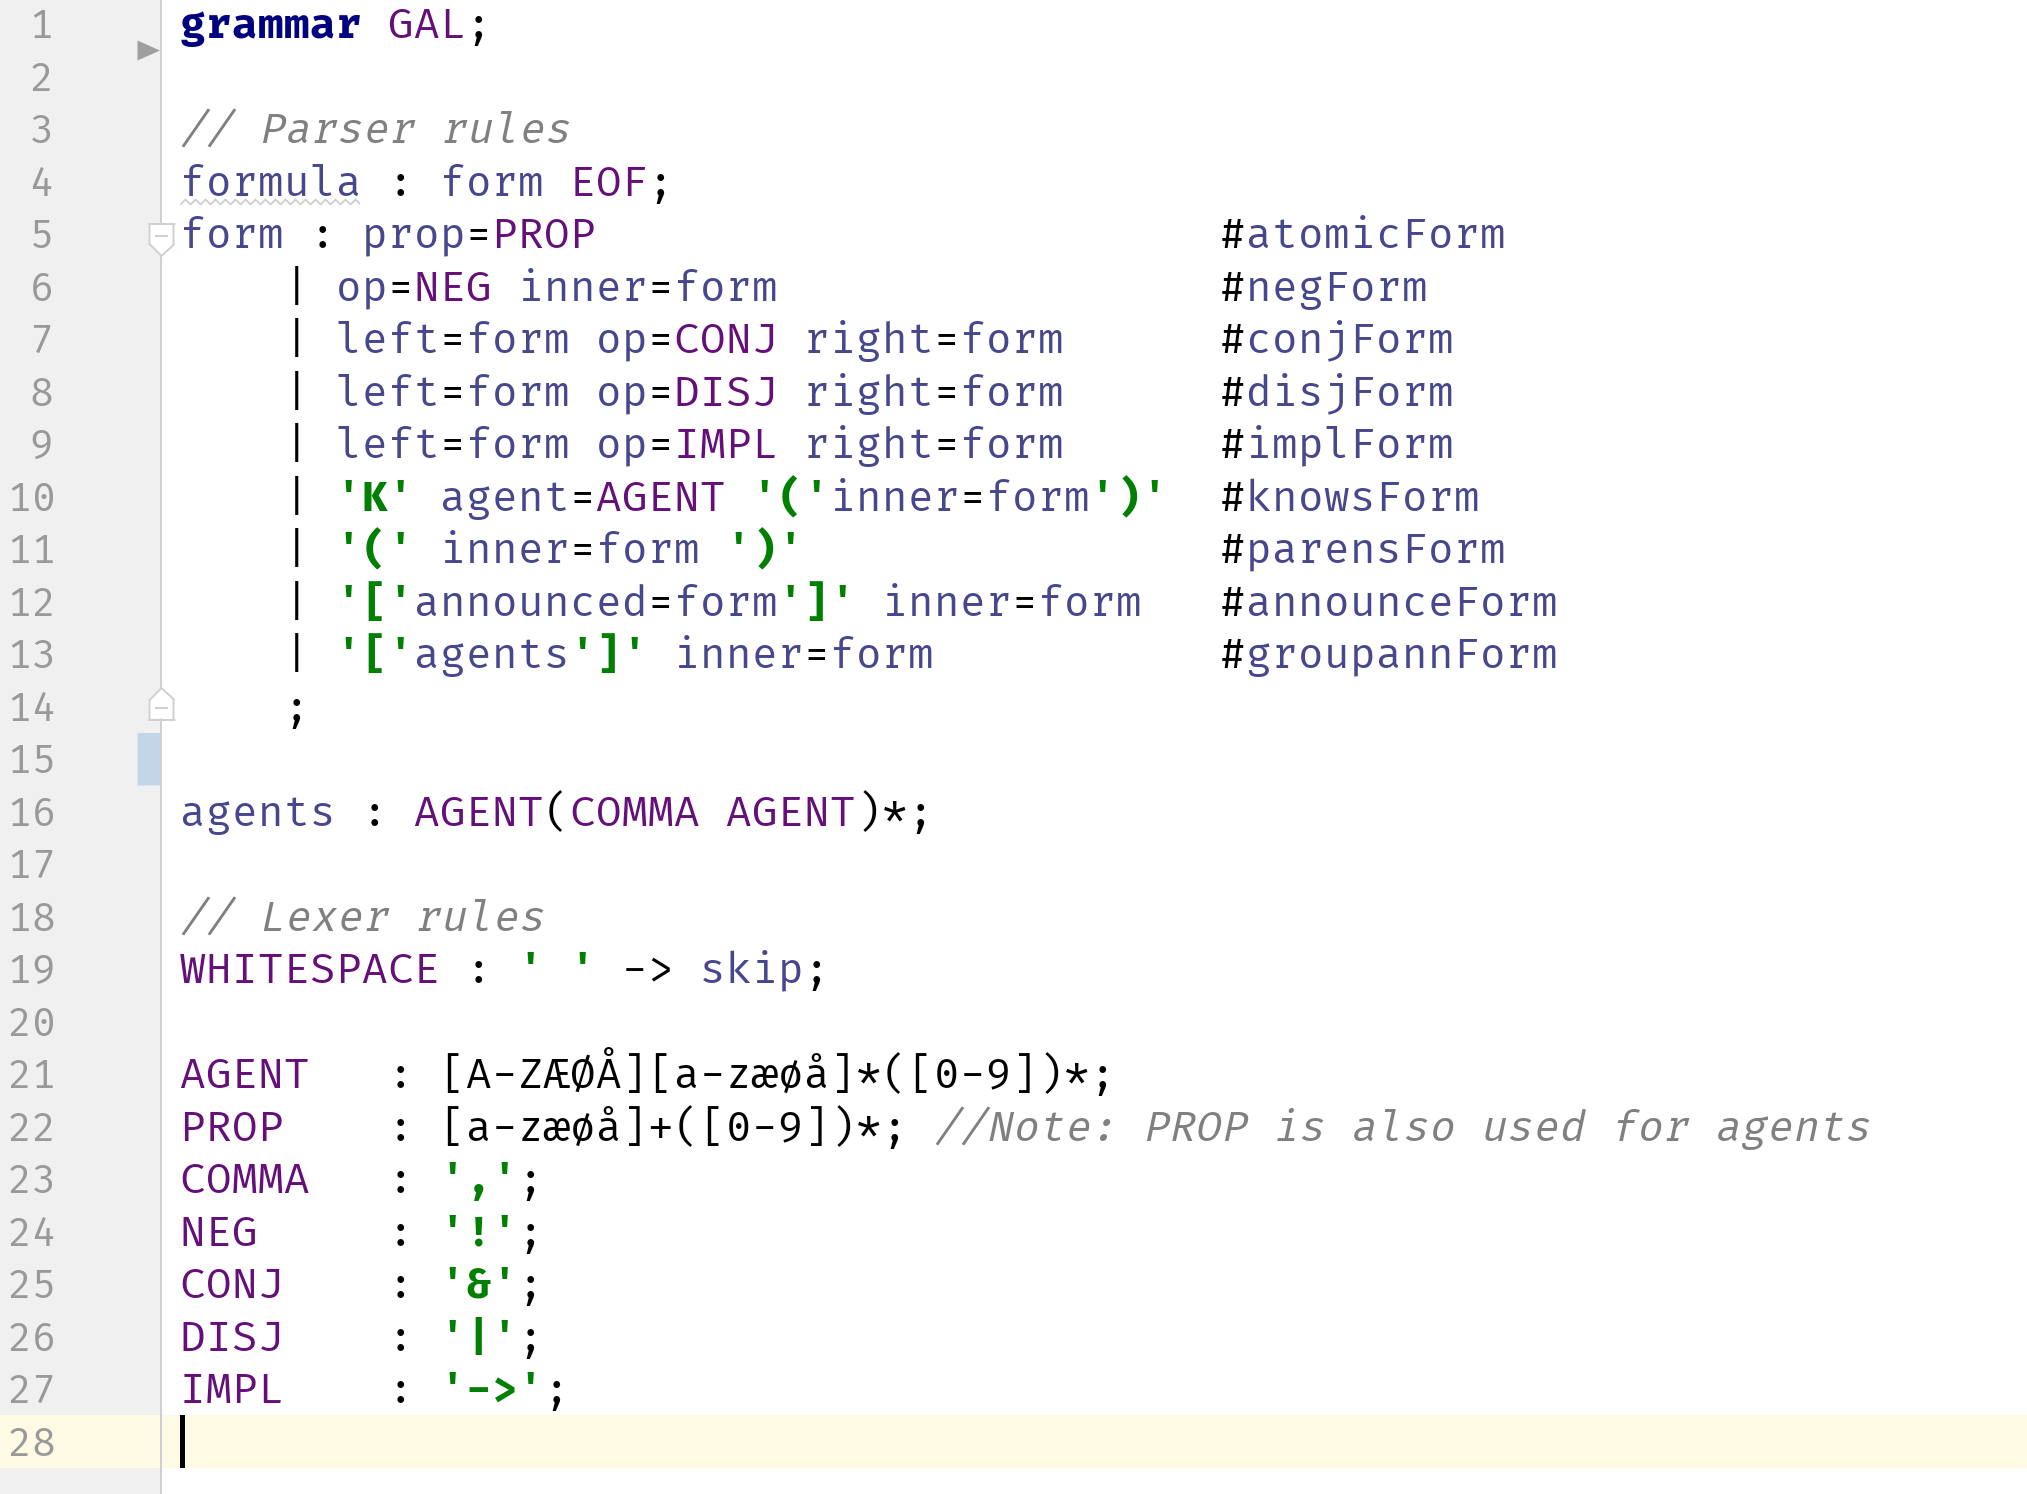
\includegraphics[width = \textwidth]{GALGrammar.png}
\end{figure}

These grammatical rules are used by ANTLR to generate parser and lexer classes which implement these rules in a manner that allow me to easily translate from raw text and lexical tokens into data structures of my own design which represent the various operators and encapsulate their semantics. One thing to note in Figure \ref{fig:grammar} are the signs used to represent negation, conjunction and disjunction. As the commonly used symbols for these operators do not exist on normal keyboards, the UI would either need extra buttons to facilitate inserting these symbols or use more easily inputable surrogate symbols. I chose the latter, going for the boolean equivalents of using exclamation marks for negations, not, ampersand for conjunctions, and, as well as the vertical bar, or `pipe' character commonly representing the or operator. Note that \cname automatically converts these characters to their `correct' symbols when displaying the input formula however, as can be seen in figure \ref{fig:debugExmpl}. 
Another small concession I had to make in order to differentiate between agents and propositions was to force agent names to be capitalized as I would otherwise have to resort to using different symbols to differentiate between regular public announcements and group announcements. Due to time constraints, the dual diamond announcement operators were not implemented, but both the grammar as well as the formula structures should be easily extendable in order to implement them as future work.

\subsection{Implementation details}

As the focus when making the application was mainly on making the it as easy to use as possible while presenting information in a visual manner that is easy to grasp, we ended up making several deviations from the logical definitions of the various structures that have been discussed throughout the thesis. Here we will discuss some of them as well as why these deviations were useful to us. Additionally we will also describe the inner workings of our tool, the technologies and frameworks it is built on as well as our reasons for choosing these.

A key difference here is how we chose to represent the components of our epistemic models themselves.  In Definition \ref{def:model} we present $\rels$ as a function from each agent to their respective equivalence relation for every state in the model, whereas in \cname we instead chose to represent these equivalence relations as a set of edges represented as objects consisting of pairs of states and sets of agents. The reasons for this ties back into how we wanted to present an interactive view of the models in our application as it felt cleaner represent each edge between states as a concrete objects which we could then bind a UI-component to, than hold onto sets of sets of states for each agent. Since each edge also has a reference to the set of agents it is valid for, it becomes trivial to visualize this information as well.

We also chose to flip the valuation function by letting states hold a reference to the set of propositions they satisfy rather than each proposition being linked to the set of states they are satisfied in. Our reasoning here is much the same as we highlight which propositions are true in which states through bindings to each state's set of propositions, which is far simpler than having to go through the entire set of propositions each time the user updates which propositions a given state satisfies. An example of how this looks can be seen in Figure \ref{fig:basicModelVis}, with both states and the edges between them being just bindings to simple data structures, updating whenever their underlying data does.

\begin{figure}[H]
	\label{fig:basicModelVis}
	\caption{A basic model, visualized in \cname}
	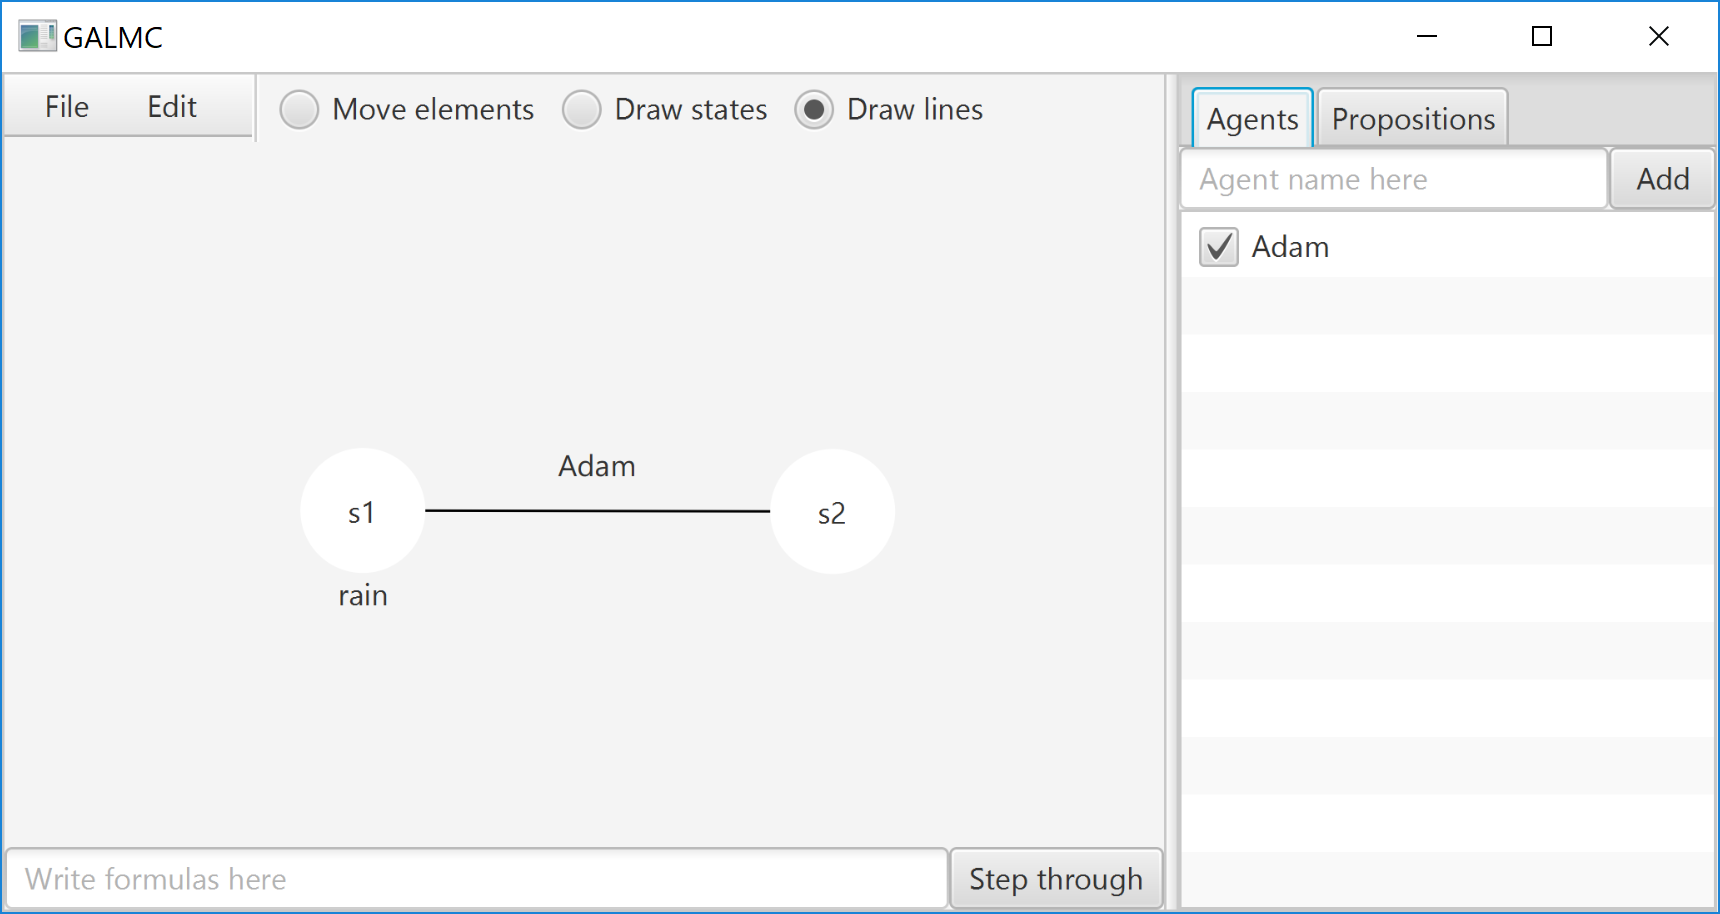
\includegraphics[width= \textwidth]{BasicModel.png}
\end{figure} 

Additionally, we also made each state aware of which edges it is connected to, trivializing the logic behind finding `neighboring' states for a given agent as we simply filter the set of edges our state is connected to based on each edge being valid for said agent and return a list of states these edges lead to.

Continuing our discussion of how we implemented our formula structures in \cname, we use a text parser generated from a small ANTLR grammar file in order to parse formulas entered by the user into a tree-like structure representing their formula. When checking this formula the user then has a choice of whether they simply want to see which states in the model satisfy their formula, or whether they want a more detailed visualization of why their formula is or is not satisfied in a specific state. If the user then opts for the first option and check their formula against the whole model, then the tool will highlight the states as either green or red, depending on whether that state satisfies the input formula. The tool also generates an interactive visual representation of the formula where the user can mouse over each operator to check the sub-formula that operator represents against the model as seen in Figure \ref{fig:labelHover}. The idea behind this being that the user might be interested in quickly seeing which states in their model satisfy the various sub-formulas to help better understand how the original operator works. The way this was implemented was to basically create UI components for each operator in the formula and the sub-formula they represent and then check each sub-formula against the model as the user mouses over them, highlighting which part of the formula they represent.

\begin{figure}[H]
	\label{fig:labelHover}
	\caption{Illustration of interactive formula display}
	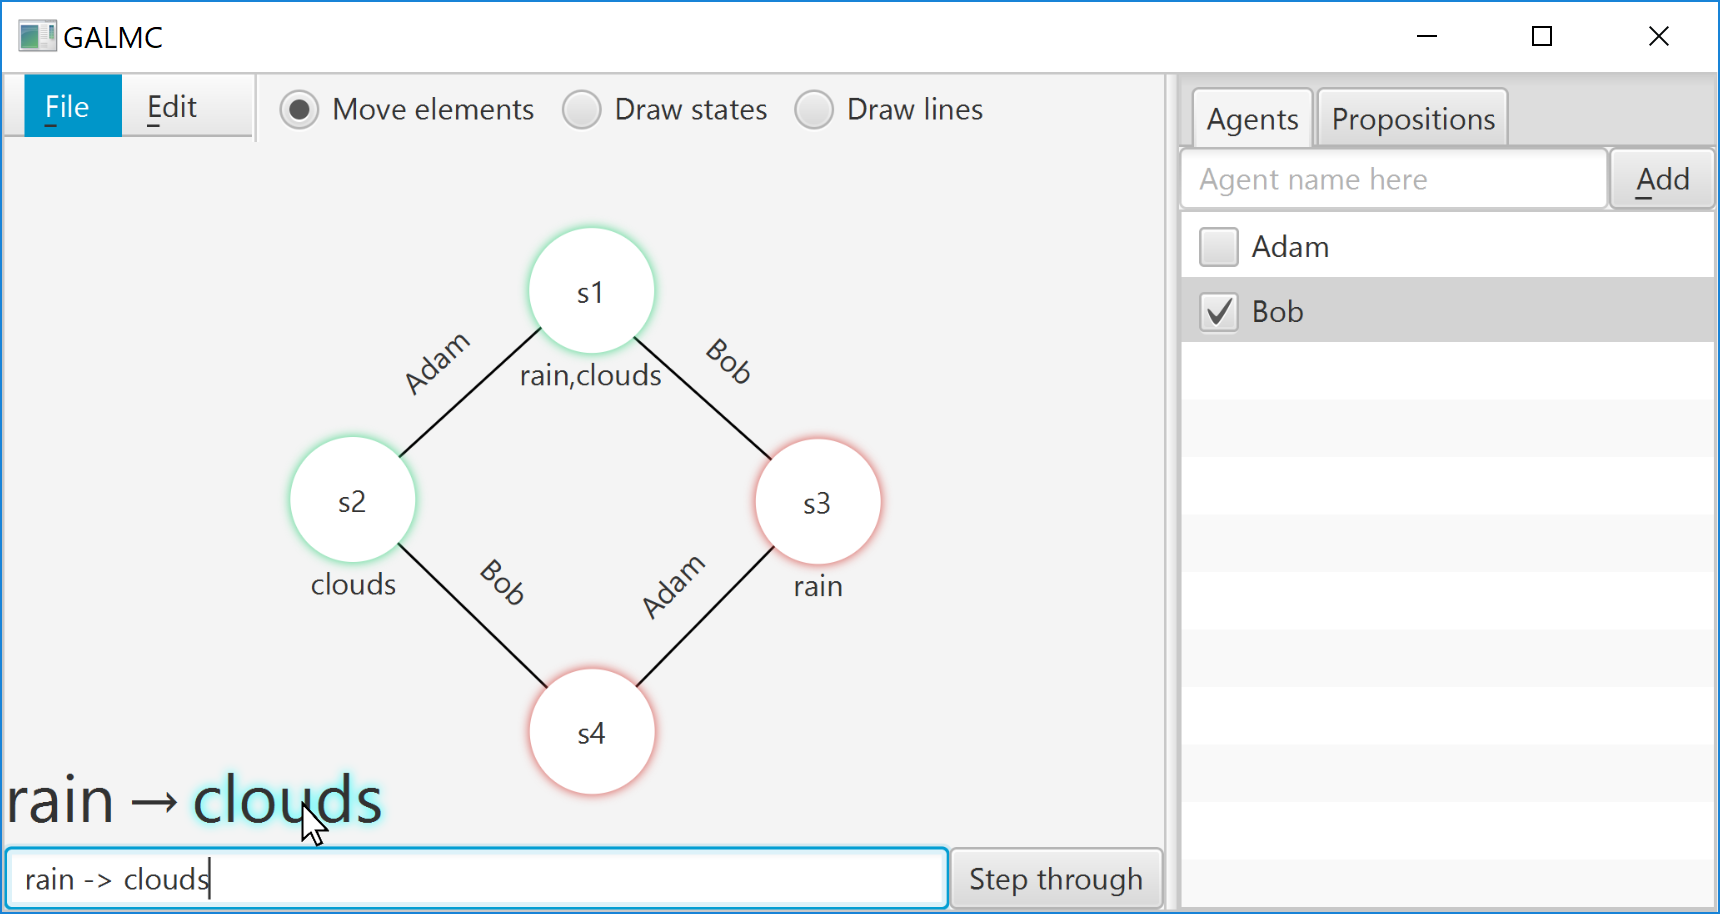
\includegraphics[width= \textwidth]{LabelMouseOver.png}
\end{figure}

How step-by-step visualization works is somewhat more involved. A high-level description of how it is implemented is that the `debugger' hooks into the $check$ function of the formula, and logs each step of the checking process. Each log then carries information about what the valuations of each operator was at that point in the process, so that this checking process can be played back and visualized in the form of showing the various operators change color as their valuations become known. One pretty cool feature of this step-by-step visualization is that it allows the user to see which states get filtered out by model updates and even see the checking process play out in each formula extension a given coalition can announce in the case of checking group announcement formulas. There were also plans for separately visualizing the set of announcements a coalition can make as well as showing what the updated models would look like, but unfortunately this had to be scrapped due to time constraints.

\begin{figure}[H]
	\label{fig:formulaImpl}
	\caption{Snippet showing how various operators are implemented}
	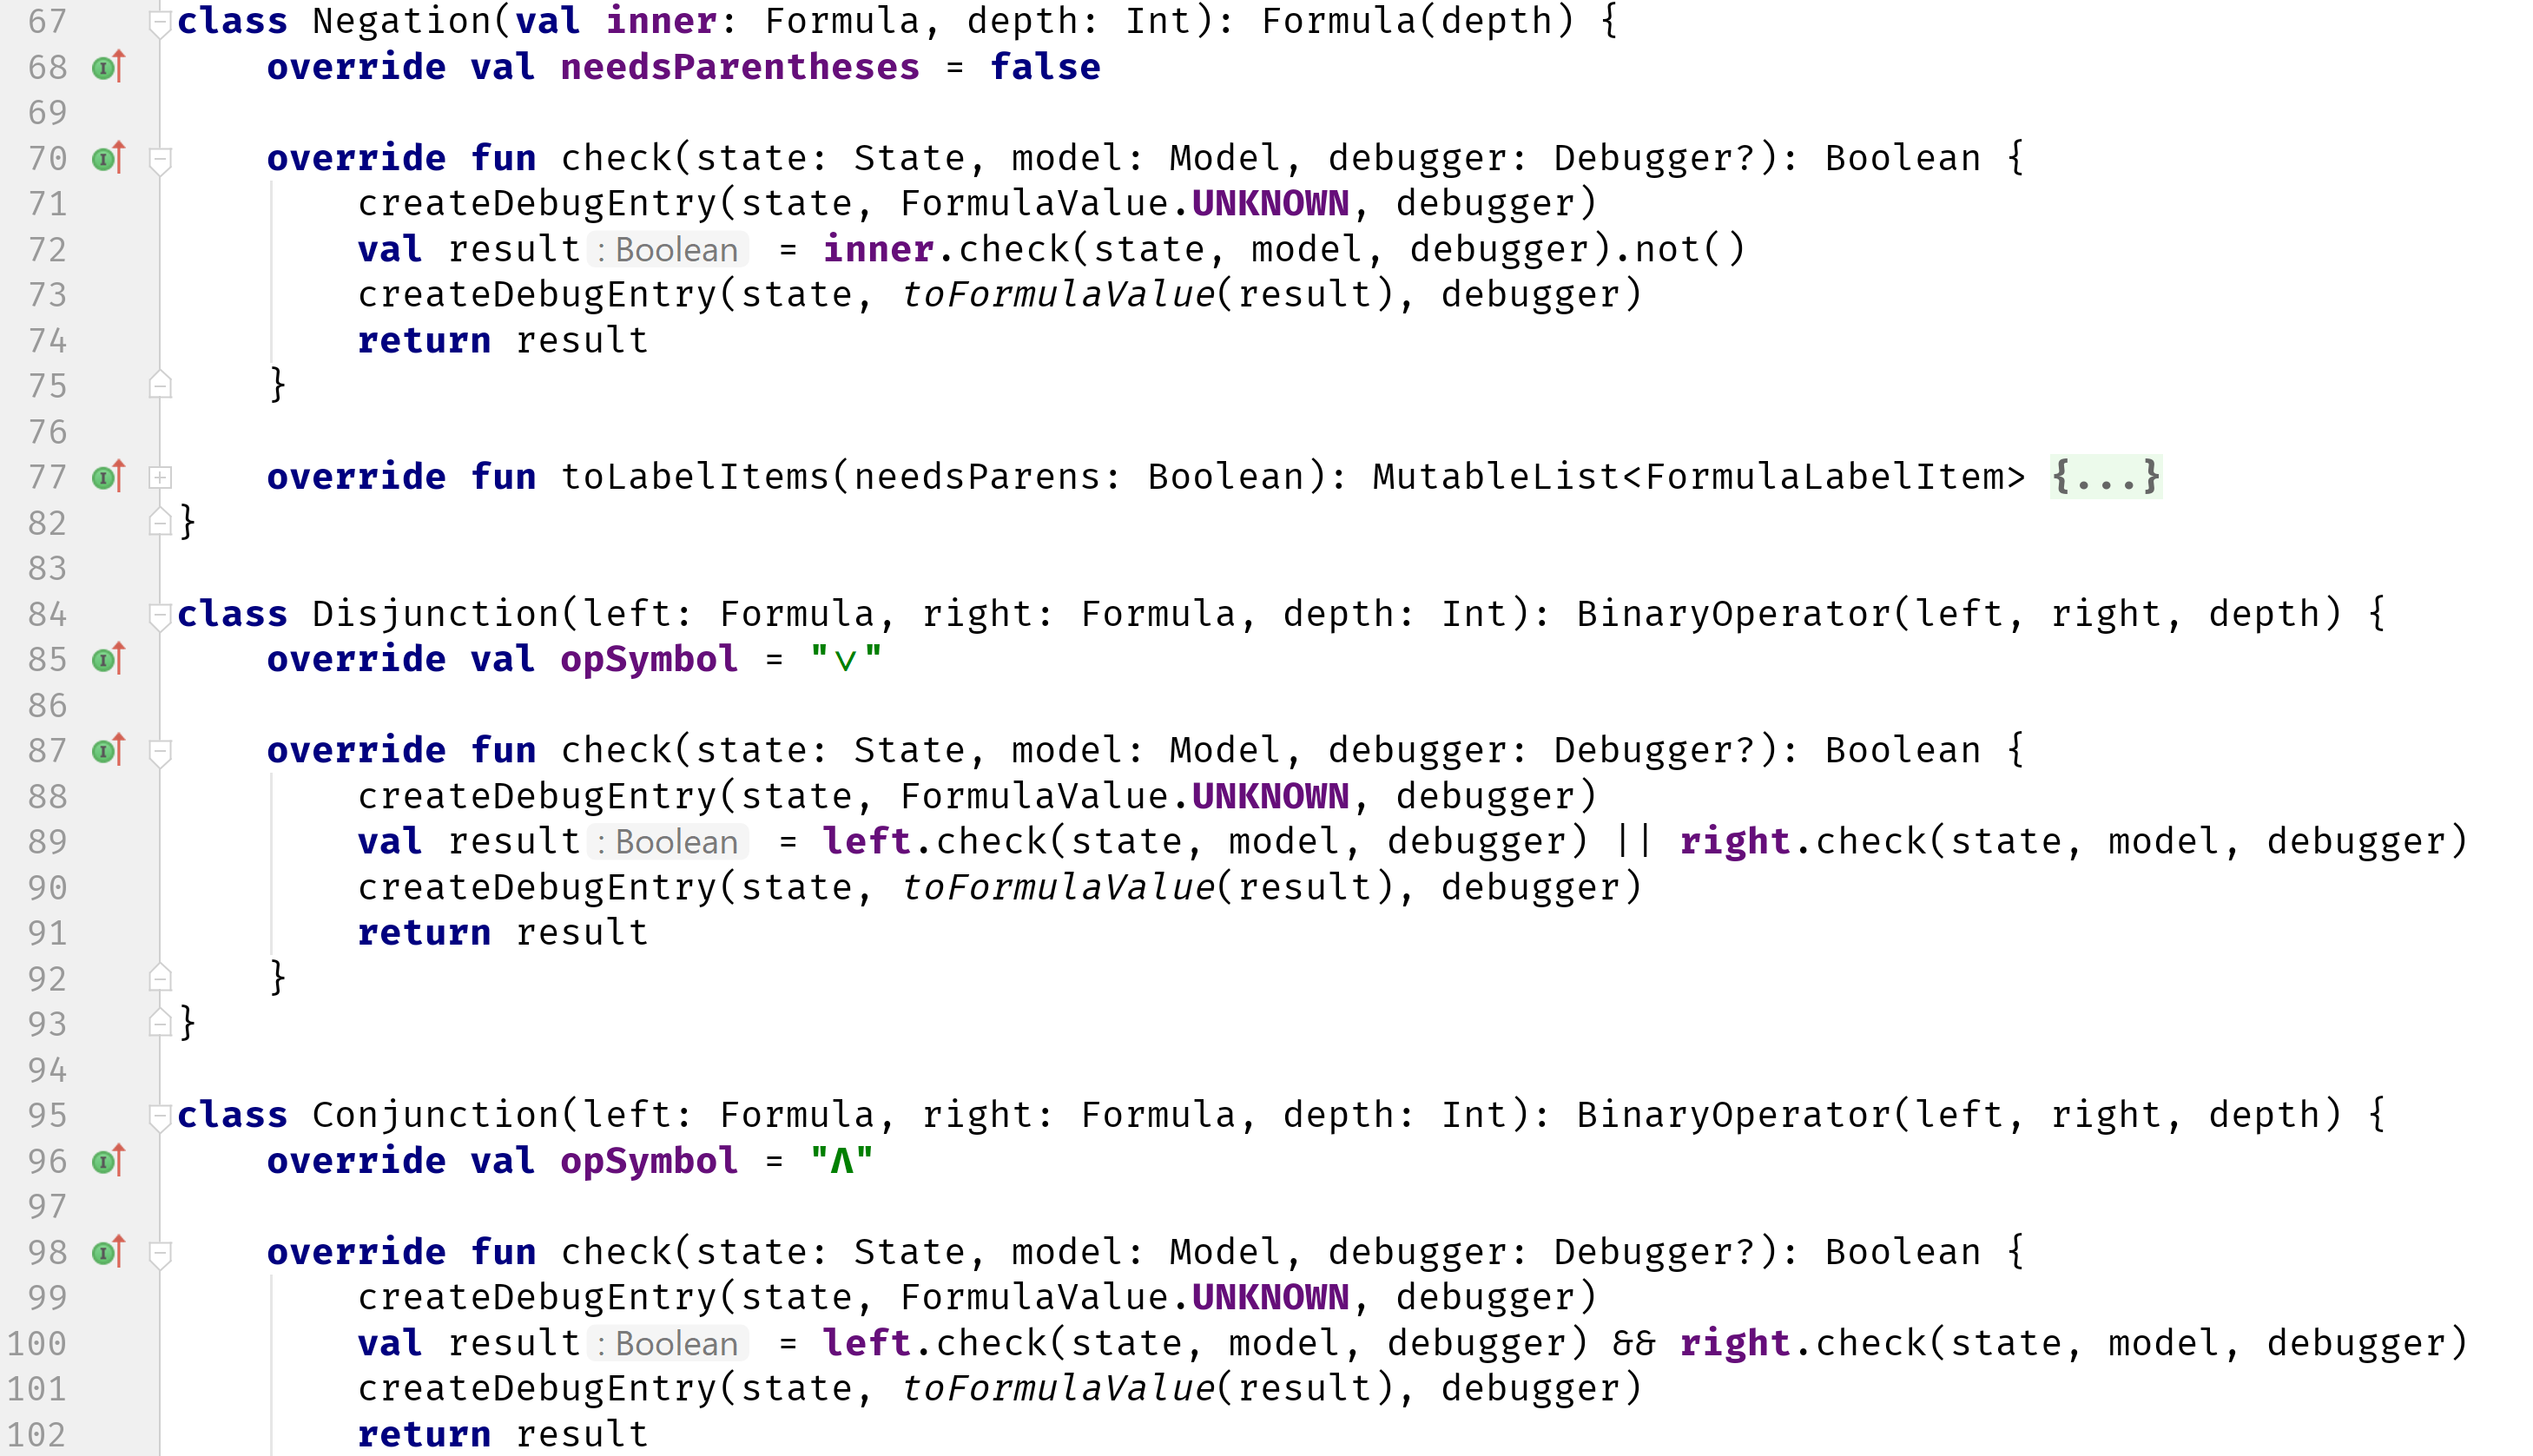
\includegraphics[width=\textwidth]{FormulaImpl.png}
\end{figure}

%Features - should explain how each of these are implemented \\\\

%Simple click-and-drag interface for creating models\\
%Reinventing the wheel in terms of click-and-drag\\
%Saving and loading models, as well as importing other models into the current model (Useful for importing commonly used components)\\
%Visualizing which states satisfy a given formula, and being able to mouse over sub-formulas to check them as well\\
%When using the step-by-step visualizer, the user can skip over sub-formulas as the application keeps track of operator depth\\

\todo{Create UML diagram of data structures and how they are connected}

%Models - $M = \{states, agents, edges, props)\}$\\

%States - 'Know about' edges they are connected to, 'know' which propositions they satisfy in order to ditch hassle of valuation function (Instead of $V(p) \rightarrow \{s\}, V(s) \rightarrow \{p\}$)\\

%Edges - Are actual objects rather than part of some equivalence relation, easier to deal with, more direct in terms of knowing what to render and interact with (Also in terms of traversing, knowing which states to interact with without having to go through a bunch of sets, i.e equivalence relations)). 'Know about' which agents they represent and which states they are between\\

%Formulas - \\

%Compare with implementations in DEMO, advantages/disadvantages of wrapping things in objects ect.\\
%We use observable objects with pointers to each other, DEMO simply has arrays of integers, which are more lightweight and potentially easier to manipulate, but much harder to render \\
%Discuss differences with logical definitions\\
%Provide walkthrough of how program checks formulas\\

%Debugger, DebugLabels, attaching itself to checking process of formulas, lots of shady voodoo to link DebugEntries in sidepanel to DebugLabels next to each state in order to update them as the user navigates through entries\\

%Debugger inserts callback into CanvasController to know when the user selects a state\\
%List of checking steps has onChange() callback telling the Debugger to apply the valuation map for that step to all formula labels\\

%Checking: Everything up to knowledge is roughly equivalent to logical definitions, minus flipped valuation function. Knowledge is similar, but instead of having an equivalence relation for each agent, each state is instead connected to other states through a set of edges which hold for a set of agents. If 


%Checking, recursive, 'logger' used to display process step-by-step\\

\subsection{Future work}

\todo{Skrive om å måle pedagogisk verdi, muligens peke ut som fremtidlig masteroppgave}

Having developed what we consider to be a potentially highly useful education tool, the big elephant in the room when discussing future work is actually measuring its educational benefit. As both user testing and educational impact studies go beyond the scope of this thesis, we certainly hope that someone might be willing to take up the torch and prove the value of \cname in such settings. While \cname is fully functional and usable as an educational aid in its current state, there are also a fair few features that we simply did not have time to implement, a few of which we will discuss.

One of the simpler additions to the tool is implementing the dual, also known as `diamond' version of the announcement operators. As these operators do not add any additional expressiveness or capabilities to the model checker they were never prioritized as they can always be expressed through the negation of the box operators. It would still be nice to have support for these operators directly however, to cut down on formula length and complexity when visualizing larger formulas. As both the ANTLR grammar and related formula components are easily extendable, implementing these operators would be fairly trivial as their underlying semantics are basically already implemented.

There are also a fair few additions to the UI we would have liked to implement, such as separately displaying the set of formula extensions a coalition can announce or provide the user with more informative error messages when attempting to parse syntactically incorrect formulas. Visualizing these formula extensions should also not prove all too challenging as the extensions are already generated when checking formulas. Similarly, the ANTLR parsers provide most of the context necessary to present inform the user of which part of their string caused an error, although more complex reasoning around how to parse ambiguous structures in regards to how to handle missing parentheses and the like might be more challenging. 

\todo{Fix apostrophe positioning somehow}\\

There were also plans for generalizing \cname{}'s model serializer in order for to be able to export the models as formats beyond its current basic binary format such as GEXF\footnote{\url{https://gephi.org/gexf/format/}} in order to be able to view these models in other tools such as Gephi\footnote{\url{https://gephi.org/}}. As the intended users of the tool are mainly students attempting to gain a better understanding of the semantics of the operators and structures in group announcement logic however, the feature was eventually scrapped as the models created would likely not be all that interesting to visualize in external tools anyway and the work involved would be fairly substantial for a feature that would probably go unused by most users.  Continuing on model serialization, we would also have liked to be able to store additional information or metadata about each model, such as being able to write notes about interesting properties a model might have or formulas that highlight said properties when checked against these models. 

